\chapter{Analiza problemu}
\thispagestyle{chapterBeginStyle}
\label{rozdzial1}

W tym rozdziale przeanalizowano problemy zawarte w tematyce niniejszej pracy oraz przedstawiono wszystkie okoliczności, w jakich system będzie funkcjonował. Omówiono podstawy gry w darta, potrzebne do zrozumienia trudności, którym trzeba sprostać przy projektowaniu i implementacji systemu. Następnie głębiej zbadano wymagania funkcjonalne, wymienione we wstępie. Zostały wprowadzone pewne matematyczne modele, które pomogą w reprezentacji rozwiązania. Podano cel stworzenia aplikacji mobilnej i jej role. Dokładnej analizie zostały poddane ograniczenia i wymagania niefunkcjonalne systemu.

\section{Gra w darta}

Dart, znany w Polsce również pod nazwą ,,rzutki'' lub ,,lotki'', jest grą, w której zawodnicy rzucają lotkami do oddalonej od nich tarczy, w celu zdobycia punktów. 

Tarcza, zazwyczaj wykonana z sizalu, znajduje się na wysokości 173 cm, w odległości 237 cm od gracza. Ma kształt koła o średnicy 45 cm i składa się z pól, którym przyporządkowane są wartości punktowe. Dzieli się ona na 20 wycinków kołowych, punktowanych od 1 do 20 (pola standardowe). Są one jednak przecięte dwoma pierścieniami: \textit{double} (zewnętrznym) i \textit{treble} (wewnętrznym). Trafienie w zewnętrzny pierścień oznacza podwojenie liczby punktów przypisanych do danego pola standardowego, a wewnętrzny -- potrojenie. Na tarczy znajdują się także segmenty \textit{inner bull}, czyli koło znajdujące się w środku, dające 50 punktów oraz \textit{outer bull} -- pierścień okalający środkowe koło, za którego trafienie przyznaje się 25 punktów. Rzut poza wymienione pola jest liczony za zero punktów. Tarcza wraz z liczbą punktów przypisaną do każdego z pól jest pokazana na rysunku \ref{tarcza_punktacja}.

\hspace{1cm}

\begin{figure}[h!]
\begin{center}
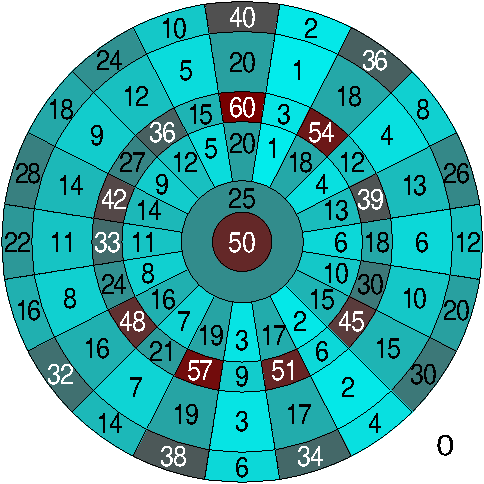
\includegraphics[width=0.4\textwidth]{obrazki/tarcza.pdf}
\end{center}
\captionsource{{\color{dgray}Tarcza do darta z przypisaniem punktów}}{Cmglee, CC BY-SA 4.0, https://commons.wikimedia.org/w/index.php?curid=49462410}
\label{tarcza_punktacja}
\end{figure} 

Najpopularniejszym wariantem darta jest \textit{501}, w którym gracze rozpoczynają rozgrywkę, mając na koncie 501 punktów. Każdy z nich wykonuje w jednej turze 3 rzuty, a suma zdobytych punktów jest odejmowana od stanu ich konta. Wygrywa ten, kto jako pierwszy osiągnie dokładnie 0 punktów. Innym znanym wariantem jest \textit{Round The Clock} -- gracze mają za zadanie trafić w każde pole na tarczy z zakresu od 1 do 20 w kolejności zgodnej z ruchem wskazówek zegara, a na końcu w pole \textit{inner bull} (tj. 20, 1, 18, \ldots, 12, 5, 50).

\section{Wykrycie rzutu i przypisanie do segmentu} \label{reprezentacja_pola}
Głównym problemem, jakim zajmuje się niniejsza praca, jest wykrycie rzutu przez system, a następnie uzyskanie segmentu, w jaki trafiła lotka. Po włączeniu systemu powinien on nieustannie analizować dane wejściowe i wysyłać sygnał, gdy rozpozna, że rzutka wbiła się w tarczę. Sygnał ten rozpocznie procesowanie danych wejściowych pod kątem obliczenia konkretnej pozycji rzutki. Najczęstszy scenariusz gry w darta wygląda tak, że każdy z graczy rzuca kolejno 3 razy, wyciąga swoje rzutki i tura przechodzi na kolejnego gracza. Z tego powodu do wygody użytkowania potrzebna jest obsługa kilku rzutów (przynajmniej trzech) bez wyciągania rzutki po każdym rzucie. Idealną sytuacją byłaby taka, gdyby bez interwencji użytkownika system był w stanie reagować na poprawne rzuty, ale ignorować wyciąganie lotek z tarczy pomiędzy turami.

Docelową daną wyjściową, którą ma dostarczać system, jest numer jednego z segmentów tarczy. W tym wypadku, zbiorem możliwych rozwiązań byłby \[W = \{0, 25, 50\} \cup A \cup B \cup C, \textrm{ gdzie } A = \{1, \ldots, 20 \}, B = \{2 \cdot a : a \in A \}, C = \{3 \cdot a : a \in A \}.\] Trzeba jednak zauważyć, że taki sposób reprezentacji powodowałby stratę pewnych informacji. Mianowicie, dla każdego $w \in (A \cap B) \cup (A \cap C) \cup (B \cap C)$  nie można by było jednoznacznie stwierdzić, jaki segment na tarczy reprezentuje. Przykładowo, pole numer 14 z podwójnego pierścienia (podwojona siódemka), byłoby tak samo przedstawiane jak standardowe pole 14. Należy zatem doprecyzować sposób reprezentacji rzutu: każdy rzut jest przedstawiany jako para $(w, t)$, gdzie $w \in W$ to liczba punktów za rzut, a $t \in \{ S, D, T \}$. $S$ oznacza pole standardowe ($\in A \cup \{0, 25, 50\}$), $D$ -- pole podwójne (\textit{double}, $\in B$), $T$ -- pole potrójne (\textit{triple}, $\in C$). Dzięki temu unika się wyżej przedstawionej niejednoznaczności: jeden segment oznacza się jako $(14, D)$, a drugi jako $(14, S)$.

Dodatkowo, przydatne może okazać się zapisanie również pośredniej reprezentacji pozycji rzutki, nie jako konkretnego pola na tarczy, ale dokładnego punktu wbicia. Nie każde rozwiązanie wymaga posiadania takich informacji, ale większość prawdopodobnie będzie je musiała wyliczyć. W takiej sytuacji punkt można przedstawiać za pomocą:
\begin{enumerate}[label=(\alph*)]
	\item współrzędnych kartezjańskich, tj. $(x, y)$, gdzie punkt $(0, 0)$ to np. lewy górny róg kwadratu opisanego na okręgu tarczy
	\item współrzędnych biegunowych, tj. $(r, \varphi)$, gdzie biegunem $O$ jest środek tarczy, a oś biegunowa $OS$ przechodzi przez punkt $S$ -- najbardziej wysunięty na prawo punkt tarczy 
\end{enumerate}
Oba podejścia są pokazane na rysunku \ref{tarcza_polozenie}.

\begin{figure}[h!]
\centering
\begin{subfigure}{.5\textwidth}
  \centering
  \includesvg[width=.8\linewidth]{obrazki/tarcza_kartezjanskie.svg}
  \caption{współrzędne kartezjańskie}
  \label{tarcza_kartezjanskie}
\end{subfigure}%
\begin{subfigure}{.5\textwidth}
  \centering
  \includesvg[width=.8\linewidth]{obrazki/tarcza_biegunowe.svg}
  \caption{współrzędne biegunowe}
  \label{tarcza_biegunowe}
\end{subfigure}
\captionsource{{\color{dgray}Rodzaje reprezentacji pozycji rzutki.}}{Opracowanie własne.}
\label{tarcza_polozenie}
\end{figure}

\section{Aplikacja mobilna}
Dodatkową częścią systemu jest aplikacja mobilna, która ma na celu atrakcyjną prezentację danych użytkownikowi, urozmaicenie rozgrywki oraz poprawę użyteczności (\textit{user experience}). W wersji podstawowej, będzie ona przede wszystkim stanowić interfejs graficzny dla systemu wbudowanego. Dzięki aplikacji mobilnej, będzie można oglądać wyniki poszczególnych rzutów oraz oglądać miejsca wbicia rzutki na wirtualnej tarczy. W rozbudowanej wersji, można do aplikacji dodać wiele innych funkcjonalności, np. wpływanie na stan gry lub wyświetlanie statystyk. 
 
\section{Ograniczenia}
Podczas tworzenia systemu należy pamiętać o ograniczeniach, które należy spełnić, by osiągnąć wszystkie wymagania, również te niefunkcjonalne. Oczywistym ograniczeniem, a jednocześnie wyznacznikiem jakości jest dokładność analizy rzutu. Może być wyrażona w różny sposób, ale ma na celu ukazanie, jak duże i/lub częste są błędy w określaniu pozycji rzutki. Bez względu na rozwiązanie, dokładność może wahać się i zależeć od wielu czynników, jednakże uśrednione dane dają natychmiastową informację o tym, na ile użyteczny jest to moduł. Głównym celem niniejszej pracy nie jest maksymalizowanie dokładności, lecz powinna być ona na poziomie pozwalającym na podstawową rozgrywkę.  

% TODO: dodać przypis do definicji czasu rzeczywistego, ew. poprawić
Innym, istotnym wskaźnikiem działania systemu jest szybkość jego działania. Jednym z celów jest możność opisania go jako \textit{system czasu rzeczywistego}. Oznacza to, że jego poprawność nie zależy jedynie od dokładności zwracanych wyników, lecz również od czasu, jaki upłynął od nadejścia danych wejściowych do otrzymania wyniku. Sytuacja z analizą rzutów odzwierciedla taką sytuację -- gracz nie chce rzucać wielu rzutek, a następnie, po czasie, zobaczyć statystyki rzutów. Aplikacja powinna działać na zasadzie akcja-reakcja: po każdym z rzutów, w krótkim czasie, powinna się pojawić informacja o wyniku. Efektem pożądanym jest sytuacja, gdy gracz nie będzie musiał czekać z następnym rzutem na zakończenie analizy poprzedniego. W przypadku, gdy oczekiwanie na wynik będzie zbyt długie, system stanie się bezużyteczny, nawet jeśli rezultaty będą bardzo dokładne. Należy zachować balans pomiędzy dokładnością a szybkością działania programu.

Rozwiązanie powinno być łatwo i szeroko konfigurowalne. Z pewnością pojawią się w nim parametry specyficzne dla np. konkretnej tarczy lub rzutek. Wszystkie tego typu części należy dobrze udokumentować oraz zapewnić prostotę modyfikacji, tak by jeden kod źródłowy mógł być z łatwością używany przez wiele osób, nawet jeśli ich lokalne parametry nie pokrywają się z tymi, które występowały u autora rozwiązania. 

Ostatnią, bardziej pragmatyczną restrykcją jest kwestia ceny całego przedsięwzięcia. Tym, co ma wyróżniać niniejsze rozwiązanie od innych jest fakt, że będzie wykonane przy użyciu łatwo dostępnych i możliwie tanich komponentów.